% for sublime text 3
%!TEX root = diss.tex

\chapter{Coherence Modeling}
\label{ch:coherence}

Local coherence modeling with varying specifications over the years is a crucial task for natural language processing. 
This chapter gives linguistic definitions related to the task that is tackled in this thesis. 


\section{Problem Definition}
\label{sec:coh-def}

In this thesis, we tackle the problem of local coherence modeling. 
The popular definition of this task is to model how sentences in a text are related to one another. 
This task has been the focus of the majority work in text processing (see Chapter \ref{ch:rel-work}). 
Variations of this task consider different types of relations, such as rhetorical \cite{hovyeduard89} or lexical \cite{morris91}, between different spans of texts, such as clauses \cite{strube.col98} or sentences \cite{halliday76}, in various text types, such as dialogue \cite{wangxinhao13} or monologue \cite{barzilay08}. 
Here we formally define the problem that is investigated in the research in this thesis.  
This definition is used to establish the next chapters of this thesis. 

\subsection{Formal Modeling}

In order to provide a formal definition of the task, i.e.\ local coherence modeling in texts, we first need to give a definition of what we refer to as a text. 
In this thesis, 
%the word ``text'' refers to a formal written and monologue sequence of sentences that transmits a meaning as a whole.  
We assume that a text consists of two sentences or more.  

\begin{definition}
Text $T$ is a sequence of finite number of sentences $[s_0, s_1, s_2, ..., s_n]$, where the number of sentences is greater than 1.   
\end{definition}

Each sentence in the above definition of a text is a list of words.

\begin{definition}
Sentence $s_i$ is a sequence of words $[w_0, w_1, w_2, ... , w_n]$ that forms a sentence structure in a text. 
\end{definition}

An underlying assumption in research on text processing is that a text is more than the sum of its sentences. 
It is not sufficient to collect an arbitrary sequence of sentences in order to obtain a text. 
Sentences in a text are supposed to be related to one another to make a whole. 
Therefore, a relationship function is required to check if a pair of sentences are related. 

\begin{definition}
Relationship function $R(s_i,s_j)$ indicates whether two sentences $s_i$ and $s_j$ in a text are related. 
The domain of this function is a pair of sentences and its range is a number. 
\end{definition} 

The output of the relation function indicates the strength of the relation between the input sentences.  
The output of this function can, however, also be limited to a binary value $\lbrace 0,1\rbrace$. 
In this case, this value indicates if there is a relationship between sentences or not. 

Having the above definition, relationships across all sentences in a text can be represented by a set $P$, which contains all relationships between any pairs of sentences in the text. 

\begin{definition}
Let $r_{ij}= R(s_i,s_j)$ indicate the relationship between a sentence pair $(s_i,s_j)$ in a text $T$; the set $P = \lbrace r_{ij}| (s_i,s_j) \in T^2, i \neq j \rbrace$ contains all $r_{ij}$ for any pair of sentences in $T$.
\end{definition}  

Although we define $P$ as a set, it can be partially structured, e.g.,\ when sentence $s_i$ has to proceed sentence $s_j$ in a text. 

While some texts can be simply recognized as coherent or incoherent, often local coherence is a matter of degree \cite{halliday76}. 
A text can be less coherent when compared to one text, but more coherent when compared to another. 
As such, since the notion of coherence is relative, coherence assessment is better represented as a ranking problem. 
Given a pair of texts, a coherence model ideally ranks the texts with respect to their coherence.
In order to rank texts with respect to their coherence, we need to capture patterns that frequently occur in more coherent texts and rarely in less coherent ones.  
Coherence patterns are templates of relationships among sentences in texts established in a way that their frequencies assist to distinguish coherent texts from incoherent ones. 

\begin{definition}
\label{def:def-coh-pattern}
A coherence pattern is a subset of relations $p \subseteq P$ occurring among sentences in a text.   
\end{definition}

We define a function to model how coherence patterns are extracted from a corpus of texts. 

\begin{definition}
Given a corpus $C$, which includes texts with different degrees of coherence, a pattern mining method $M$ extracts all subsets of relations that occur in any text in $C$ as a set of coherence patterns. 
\end{definition} 

The output of the pattern mining process on a corpus of texts is a set of coherence patterns. 
The coherence of a text can be modeled by a vector of frequencies of these patterns in the text. 

\begin{definition}
Let $P=\lbrace p_0,p_1,p_2,...,p_m \rbrace$ be a set of extracted patterns from a corpus of texts $C$; the perceived coherence of text $T$ is represented by  vector $\phi = <f_0, f_1, f_2,...,f_m>$, where $f_k$ is the frequency of pattern $p_k$ in text $T$. 
\end{definition}

Having a vector representation of coherence lets us employ machine learning models to rank texts. 
In Chapter \ref{ch:rel-work}, we describe different approaches to modeling relationships between a pair of sentences, i.e.\ $R(s_i,s_j)$, and how they represent the set of all relations in a text, i.e.,\ $P$.  
There, we also review how method $M$ is derived by different computational models. 
We employ a powerful representation for texts, i.e.\ the entity graph representation \cite{guinaudeau13}, from the literature and develop our approach for extracting coherence patterns in Chapter \ref{ch:coh-patterns}. 
We further improve the predictive power of coherence patterns by a new approach to relationship representations among sentences, i.e. $P$, in Chapter \ref{ch:lex-graph}. 

\section{The Linguistics of Coherence}

The aforementioned formal definition of the problem is sufficient for the research in this thesis to develop a representation of cohesive relations in a text, and to extract coherence patterns. 
However, since coherence is a semantic property of texts, the definition needs to be related to linguistic properties of texts. 

Our aim is to develop an approach which provides a representation of the coherence of a text. 
Therefore, we need to understand what aspects of sentences serve to relate sentences and how coherence patterns are modeled in linguistics of coherence. 
In order to accomplish this, we explain related linguistic properties that are required to complete our definition. 


\subsection{Text}

The first definition in our formal model of coherence is about text. 
In linguistic research, the word ``text'' is used to refer to any passage, spoken or written, of whatever length that forms a unified whole \cite{halliday76}. 
In this thesis, we follow other coherence models \cite{barzilay08,guinaudeau13} and use the word ``text'' to denote a merely monologue written passage, which includes more than one sentence.
One-sentence texts, of course, do exist, such as public notices, proverbs and advertising slogans.  
For instance, a sample text with only one sentence is shown in Example \ref{ex:coh-one-sent-text}\footnote{Taken from \url{https://www.engvid.com/english-resource/50-common-proverbs-sayings/}, accessed 1 June 2018.}: 

\begin{examples}
    \label{ex:coh-one-sent-text}
    A journey of a thousand miles begins with a single step.
\end{examples}

However, in the research of this thesis\footnote{Texts that consist of one sentence do not exist in the datasets employed for experiments of the research in this thesis.}, we assume that texts contain at least two sentences. 
We also assume that texts are written in a formal language, in contrast to an informal language like what is used in tweets\footnote{A post made on the social media application Twitter.}. 

\subsection{Coherence}

Coherence is a crucial factor of a well-written text. 
It makes the text distinguishable from an unrelated sequence of sentences. 
A coherent text discusses a sequence of topics in a structured way in which a reader can recognize and relate to one another, and collectively render a coherent text as a unified whole \cite{stede12}. 
Each topic tends to occupy a (topical) segment of the text \cite{hearst97}. 
Coherence is defined based on the relations and structures of topical segments in a text. 
This structure is sometimes referred to as global coherence since it is coarse-grained and spans the entire text \cite{elsner07}. 
\newcite{lautamatti78} defines the term ``topic'' as what sentences are about and the term ``comment'' as information about the topic.  
In general, however, it is not straightforward, first, to define the notion of topics and then to recognize topics and their boundaries across text segments \cite{stede12}.
However, we review some computational topical coherence models in Chapter \ref{ch:rel-work}. 


\subsection{Local Coherence}

From the linguistic viewpoint, a coherent text employs linguistic devices, more readily identifiable linguistic signals, to relate sentences of a text to each other. 
These devices signal readers to interpret each sentence while considering its relations with other linked sentences \cite{vandijk77}. 
Therefore, understanding the text implies uncovering these relationships.  
\textcolor{red}{The way that linguistic devices are used to relate sentences in a text is known as local coherence.} 
In some literature in text linguistics, e.g.\ \newcite{halliday76}, this phenomenon is referred to as cohesion.   
\newcite{stoddard91} argues that local coherence and cohesion are not distinguishable and can be used interchangeably. 
\newcite{stede12} states that signals of local coherence serve as indicators of topic continuity; consequently, the absence of a surface relation is a sign of a topic shift. 
Since the research in this thesis is about local coherence modeling, henceforth in this thesis it is referred to as ``coherence modeling''. 
We explicitly distinguish them where they are not distinguishable from the context. 

Prominent cohesive devices can be grouped in grammatical and lexical relations between elements of sentences \cite{halliday76}. 
Grammatical relations are reference, substitution, ellipsis and conjunctions. 
Lexical relations include any lexical-semantic relation, such as repetition, synonym, antonym, and the like, between words of sentences. 
Among the grammatical relations, reference cohesive devices are also known as entity-based relations. 
The intuition behind the leveraging entity relations for coherence modeling is that related sentences in a text keep referring to the same entity. 
Following \newcite{barzilay05a} and \newcite{elsner10}, we define an entity as follows: 

\begin{definition}
    An entity is perceived as a person, a physical object, a concept, or an abstraction that exists (or may exist) in the world external to a text.  
\end{definition}

An entity can be referred to in different ways by various referral expressions, or mentions. 

\begin{definition}
	Pieces of a text that are used to refer to an entity are called mentions. 
\end{definition}

Having these definitions, one way of representing an entity is to group all mentions that refer to that entity. 
Each cluster of mentions 
%, which can be imagined as a bucket containing all referent mentions,
represents an entity. 
The task of identifying mentions that refer to the same entity is known as coreference resolution.   
%The goal of this task is to cluster mentions of a text based on entities that they are referring to.  

\begin{definition}
	The task of detecting all mentions in a text and clustering all mentions that refer to same entities is called coreference resolution. 
\end{definition}

 
The sample text in Example \ref{ex:coh-ref}\footnote{Taken from \url{https://web.stanford.edu/class/archive/cs/cs224n/cs224n.1162/handouts/cs224n-lecture11-coreference-6up.pdf}, accessed 2 June 2018.} shows how entity-based relations link sentences. 

\begin{examples}
	\label{ex:coh-ref}
	\textbf{Mr.\ Obama} visited the city. \\
	\textbf{The president} talked about Milwaukee’s economy. \\
	\textbf{He} mentioned new jobs. \\
\end{examples} 

\emph{Mr.\ Obama}, \emph{The president} and \emph{He} are three mentions that refer to the 44th president of the United States. 
Three sentences of the text shown in Example \ref{ex:coh-ref} are connected because they contain mentions that refer to the same entity. 

One of the popular entity-based frameworks for local coherence modeling is the Centering Theory \cite{grosz95}. 
The core of this theory is the concept of the text center. 
The center at any given point in a text is the most salient entity at that point. 
For instance, in the text that is shown in Example \ref{ex:coh-ref}, the center is on the entity ``Barack Obama''.
The center captures the focus of attention in the reader's mind \cite{grosz95} as the text progresses. 
The centering theory accounts for the process of center flowing in a text. 
The original centering theory (for English texts) sees the grammatical roles of the mentions of entities in sentences as the most important linguistic signs of saliency of entities. 
Specifically, the grammatical subject is taken as the default position for the text center. 
Depending on the configuration of grammatical roles in adjacent sentence, \newcite{brennan87} define four different types of transitions for the text center across sentences of a text. 
These transitions capture the smoothness of the center move from one sentence to another. 
When a sentence focuses on the topic, i.e.\ the center, which is discussed in sentences preceding that sentence, then the transition is Retain or Continue; the other types of transitions involve a topic shift: Smooth Shift, and Rough Shift. 
The idea of the centering theory has been applied directly in models of coherence \cite{karamanis04a}.  
However, since it requires human annotations for center transitions between sentences, some models employ the basic principles of the centering theory as soft constraints or features in a probabilistic framework. 
An example of such models is the entity grid model \cite{barzilay05a,barzilay08}, which will be discussed in more detail in Chapter \ref{ch:rel-work}.

Further research shows that grammatical role information is far less predictive for tracking the text center in German, as it is a free word order language \cite{strube.acl96}. 
Instead, the functional information structure is considered \cite{danes74}.  
This structure captures flows between given information and new information in a text. 
Some information in a sentence is known or old because it is discussed by preceding sentences, and some information is new. 
The functional information structure is explained by \newcite{halliday76} as \mbox{theme-rheme} relations in a text. 
Theme can be taken as given information, as a point of the text departure, and rheme is (almost) similar to new information, as clarification information about the theme. 
While theme conveys information that is initially introduced in text, rheme presents specific 
information about the theme. 
As the theme-rheme movement continues through a text, ideas in the text are expected to flow along smoothly and be easy for readers to understand. 
Thematic relations between sentences in texts reveal some patterns \cite{danes74}, which are called coherence patterns.
In Chapter \ref{ch:coh-patterns}, we define our approach to coherence pattern mining and provide more explanation about functional information structure \cite{danes74} in texts. 

The other perspective of local coherence is lexical cohesion. 
It is the cohesive effect based on \mbox{lexico-semantic} relations between words in a text. 
An advantage of lexical cohesion models, in contrast to \mbox{entity-based} models, is that it requires no annotation because lexicons are directly accessible from a text. 
The insight of local coherence resulting from lexical relations is that content words in a text do not occur independently of one another but rather bear semantic similarity because of the common topic. 
A form of lexical cohesion is reiteration, which involves different types of lexical relations such as repeating a word, using a synonym of a word, and employing a superordinate word. 
Example \ref{ex:coh-lex} is taken from \newcite{halliday76} to illustrate these relations:

\begin{examples}
	\label{ex:coh-lex}
	(a) Repetition: There was a large \textbf{mushroom} growing near her, about the same height as herself; and when she had looked under it, it occurred to her that she might as well look and see what was on the top of it.\\
	She stretched herself up on tiptoe, and peeped over the edge of the \textbf{mushroom}, [...] 

	(b) Synonymy: Accordingly [...] I took leave, turned to the \textbf{ascent} of the peak. \\
	The \textbf{climb} is perfectly easy. 

	(c) Superordinate: Henry's bought himself a new \textbf{Jaguar}. \\
	He practically lives in the \textbf{car}. 

\end{examples} 

In Example \ref{ex:coh-lex}(a), the word ``mushroom'' is exactly repeated. 
In (b) two words ``ascent'' and ``climb'' carry the same meaning. 
In (c), the word ``car'' is a superordinate, any word whose meaning includes that of the earlier one, of ``Jaguar'', as vehicle is a superordinate of the car. 
The relationship between ``spoon'' of ``teaspoon'' is another example of the superordinate relation. 
The boundary between the reiteration type of lexical cohesion and reference type in entity-based relations is by no means clearcut
%\footnote{However, properly speaking, reference is irrelevant to lexical cohesion. As we discuss later lexical cohesion relationship between two items does not need to imply a coreferent relationship.} 
\cite{halliday76}. 
This clarifies why for purposes of the research in this thesis, local coherence and cohesion are largely synonymous.

It is not necessary for two lexical occurrences to be coreferent in order to make a cohesive relation.  
For instance, consider Example \ref{ex:coh-nonref} taken from \newcite{halliday76}(p.~282). 
The word ``boy'' in the question and the word ``boys'' in the answer (a) are not coreferent; however, their semantic relationship serves to link the sentences. 
This relationship is not in any way dependent on the presence of other words in the sentence; it is not the wriggling in (a) that provides the context for the context, as the answer (b) shows. 

\begin{examples}
	\label{ex:coh-nonref}
	Why does this little \textbf{boy} have to wriggle all the time? \\
	(a) Good \textbf{boys} don't wriggle. \\
	(b) \textbf{Boys} should be kept out of here. \\
\end{examples} 

\textcolor{red}{
This leads to a systematic relationship between a pair of words because the words frequently occur in similar textual context. 
For instance, words ``boy'' and ``girls'' in Example \ref{ex:coh-collocation}\footnote{The text is taken from \cite{halliday76}(p.~285)} relate the sentences, although they are neither coreferent nor even synonym. 
}
\begin{examples}
	\label{ex:coh-collocation}
	Why does this little \textbf{boy} have to wriggle all the time? \\
	\textbf{Girls} don't wriggle. 
\end{examples}

In summary, there is a local coherence relation between any pair of lexical items that stand to each other in some lexico-semantic relations. 
This includes any type of relations, such as relations between word pairs shown in Example \ref{ex:coh-word-pairs} \cite{halliday76} (p.~285). 

\begin{examples}
	\label{ex:coh-word-pairs}
	rail ... road \\
	car ... brake \\
	try ... succeed \\
	walk ... drive \\
	Tuesday ... Thursday \\
	like ... hate \\
	red ... green 
\end{examples}

For textual purposes, it is (almost) sufficient to know that a pair of words are in a relationship, rather than the type of relation \cite{halliday76}. %(p. 285).  
\newcite{hoey91} examines how lexical cohesive elements make a text organized and contribute to local coherence. 
He shows that relations between semantically related words in a text follow similar patterns in texts. 
In Chapter \ref{ch:rel-work}, we survey some related computational models of lexical cohesion in texts. 


\subsection{Coherence Patterns}

\textcolor{red}{An increasing number of researchers and practitioners in natural language processing face the prospect of having to work with entire texts rather than individual sentences. 
}
While it is clear that text must have useful structure, its nature is less clear, making it more difficult to exploit in applications \cite{webber12a}. 
A text commonly comprises a sequence of sentences. 
Within a text, the patterns formed by its sentences mean that the whole text conveys more than the sum of its separate parts. 
Text structures are the patterns that one sees in \mbox{multi-sentence} texts \cite{webber12a}. 
Recognizing these patterns in terms of the elements that compose them is essential to correctly deriving and interpreting information in the text. 
%The elements may be topic, each  about a set entities and what is being said about them.
A text can be structured by its topics, each comprising a set of entities and a limited range of things being said about them. 
Patterns of coherence relations can also be characteristic of particular types of text and therefore be of value in assessing the quality of automatically generated text. 

The concept of coherence patterns is linguistically derived from the texture of texts. 
\newcite{stoddard91} defines a text as ``a phenomenon of seemingly infinite complexity due to its synergistic nature'' where elements of a text are supposed to corporate together for an enhanced effect. 
It is synergism that makes texts more than sequential words and sentences. 
The dynamic of synergism, which is because of its multi-dimensionality, is beyond the linear, sequential structure of texts. 
One cause of the multidimensionality of synergism is a global component which can be referred to as ``texture'', which is the quality created by the combination of the different elements in a text \cite{stoddard91}. 
\textcolor{red}{Indeed, one of the preliminary principles of texture is coherence, which is a type of unifying device which we construct consciously or unconsciously as we process texts \cite{halliday76}.}

From \newcite{stoddard91}'s perspective, the texture of texts is interpretable by means of elements that are common in all texts and those that discriminate texts. 
These elements are referred to as patterns of coherence. 
\newcite{stoddard91} believes that the texture property of texts manifests itself in patterns of coherence in written texts. 
It is worth noting that texture, in one sense, involves the quality of depth, which may range from minimal (approximating ``flatness'') to maximal, or at any level in between. 
In other words, patterns of coherence can be as basic as the linear order of elements of a text or be more complicated by incorporating relations between non-adjacent sentences. 
Incorporating non-adjacent relations yield non-linear patterns. 
\newcite{stoddard91} describes the texture of texts as a composite of patterns -- storyline patterns, rhetorical patterns, linguistic patterns and so on -- which when overlaid to create the totality of a text creates variant textures which are like the ``fingerprint'' of a text. 
In this sense, the texture of texts is more closely related to ``style'', which is certainly related to local coherence \cite{barzilay08}. 

%Other linguistics also relate what we call coherence patterns to the texture or the nature of texts. 
\newcite{halliday76} claim that ``linguistic patterns  [...] embody, and at the same time impose structure on our experience of the environment [...]''.
Because of this, they suggest that patterns help readers to understand a text as coherent and consistent with our knowledge, experience, and environment. 

One factor that must be considered in describing coherence patterns as the input to texture is the likelihood of patterns occurring over the large stretch of a text \cite{stoddard91}.  
The unity of texts happens because readers perceive the interactiveness of ``text components''. 
Because these appear to have a degree of consistency across all texts, they should be identifiable as texture-forming mechanisms.
Moreover, this would be easier for readers to smoothly process texts in which the patterns of interactiveness among components are familiar to the reader.  

\newcite{stoddard91} illustrated the patterns of cohesion and the way that the patterns interact graphically for a few texts. 
The term of ``networks of cohesion'' proposed by \newcite{halliday76} can be interpreted (almost) equivalent to this graphical illustration. 
The results of text analysis in \newcite{stoddard91} show that local coherence leads to connectivity patterns.
She suggests to unify a text by means of coherence network patterns that span varying lengths of text passages. 
The importance of the results lies in the fact that typologies (i.e.\ graphical structure) and counting, when supplemented with other kinds of analysis, give us a better understanding of local coherence as it contributes to the texture of a text. 

The facts that cohesive patterns occur in texts and cohesiveness is relative in texts provide useful validation of the intuition used in the research presented in this thesis: Coherent texts reveal some regularities in their structure that can be encoded by the frequency of coherence patterns. 
All of this linguistically supports our first research question that is concerned with \mbox{non-linearity} of patterns. 

Another piece of in linguistic research related to coherence patterns is performed by \newcite{danes74a}. 
He describes the structure of texts by the concept  of ``thematization'' that has been also noticed by \newcite{halliday76} as ``information focus'' or \mbox{given-new} information. 
\newcite{halliday76} summarize it in this way: ``given information'' has been talked about in a text and ``new information'' is been mentioned now.  
Similarly, theme, from \newcite{danes74a}'s point of view, is the point of departure where the text flows from a topic (``given information'') towards another topic (``new information''). 
In simple words, theme can be realized as ``given information'' and rheme is ``new information'' and ``thematization'' is about patterns of transitions between themes and rhemes in a text. 

The contextual determination of givenness is far from being a simple phenomenon \cite{danes74a}. 
Tentatively, some information that is mentioned directly or indirectly in a text can be interpreted as given information. 
\newcite{danes74} explains that ``given information'' can be realized either directly with an identically wording expression or indirectly with a synonymous one.   
The indirect mentioning is based on semantic inference. 
For instance, the expression ``illness'' occurring in a sentence might convey a piece of given information if in one of its preceding sentences ``disease'' has been somehow mentioned. 
In contrary, the new information may either not be mentioned in its proceeding context or be related to given information. 
This phenomenon is known as the relation between ``theme'' and ``rheme'' in \newcite{danes74a} as is shown by  $T \rightarrow R$. 
This illustrates that the flow of information is from ``given information'' (or ``theme'') to ``new information'' (or ``rheme'').
\newcite{danes74a} states that the inquiry into the thematic organization of the text is closely connected with the investigation of the so-called ``text coherence'' or ``text connectivity''.
He analyzes Czech scientific and other professional texts, as well as some tentative soundings in the area of German and English language materials.
He ascertains several major types of organizational patterns in examined texts, represented in Table \ref{tab:danesh_coherence_patterns}. 


\begin{table}
	\begin{center}
		\begin{tabular}{c|c}
		\toprule
		\textbf{Pattern ID} & \textbf{Pattern} \\
		\midrule
		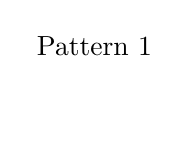
\begin{tikzpicture}
			\node [] (n0)  at (0.0,0.0) {};
			\node [] (n1)  at (0.0,1.0) {Pattern 1}; 
		\end{tikzpicture} 
		&
		\begin{tikzpicture}
			\node [] (n1)  at (0.0,2.0) {$T_1 \rightarrow R_1$}; 
			\node [] (n2)  at (1.8,1.0) {$T_2 (= R_1) \rightarrow R_3$};
			\node [] (n3)  at (4.2,0.0) {$T_3 (= R_2) \rightarrow R_4$}; 
			\draw[->] (0.5,1.7) -- (0.5,1.3);
			\draw[->] (3.0,0.7) -- (3.0,0.3);
		\end{tikzpicture}

		\\
		\midrule
		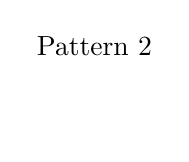
\begin{tikzpicture}
			\node [] (n0)  at (0.0,0.0) {};
			\node [] (n1)  at (0.0,1.0) {Pattern 2}; 
		\end{tikzpicture} 
		 &
		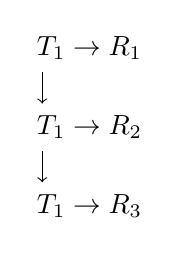
\begin{tikzpicture}
			\node [] (n1)  at (0.0,2.0) {$T_1 \rightarrow R_1$}; 
			\node [] (n2)  at (0.0,1.0) {$T_1 \rightarrow R_2$};
			\node [] (n3)  at (0.0,0.0) {$T_1 \rightarrow R_3$}; 
			\draw[->] (-0.6,1.7) -- (-0.6,1.3);
			\draw[->] (-0.6,0.7) -- (-0.6,0.3);
		\end{tikzpicture}

		\\
		\midrule
		\begin{tikzpicture}
			\node [] (n0)  at (0.0,0.0) {};
			\node [] (n1)  at (0.0,2.0) {Pattern 3}; 
		\end{tikzpicture} 
		&
		\begin{tikzpicture}
			\node [] (n0)  at (2.2,4.0) {$[T]$}; 
			\node [] (n1)  at (0.0,3.0) {$T_1 \rightarrow R_1$}; 
			\node [] (n2)  at (1.8,2.0) {$T_2 \rightarrow R_2$};
			\node [] (n3)  at (4.2,1.0) {$T_3  \rightarrow R_3$}; 

			\draw[->] (n0.south) -- (-0.5,3.3);
			\draw[->] (n0.south) -- (1.3,2.3);
			\draw[->] (n0.south) -- (3.5,1.3);
		\end{tikzpicture}

		\\
		\midrule

		\begin{tikzpicture}
			\node [] (n0)  at (0.0,0.0) {};
			\node [] (n1)  at (0.0,2.0) {Pattern 4}; 
		\end{tikzpicture} 
		&
		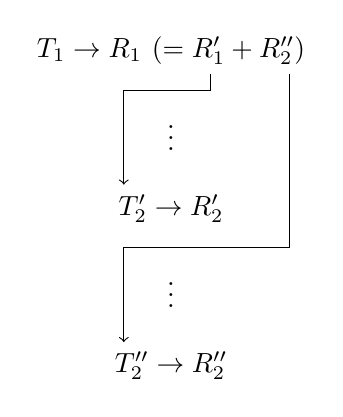
\begin{tikzpicture}
			\node [] (n0)  at (0.0,4.0) {$T_1 \rightarrow R_1\textit{ }( = R_1^\prime + R_2^{\prime\prime} )$}; 
			\node [] (d0)  at (0.0,3) {$\vdots$}; 
			\node [] (n1)  at (0.0,2) {$T_2^\prime \rightarrow R_2^\prime$}; 
			\node [] (d0)  at (0.0,1) {$\vdots$}; 
			\node [] (n2)  at (0.0,0.0) {$T_2^{\prime\prime} \rightarrow R_2^{\prime\prime}$};
			\draw [->] (0.5, 3.7) -- (0.5, 3.5) -- (-0.6, 3.5) -- (-0.6, 2.3);
			\draw [->] (1.5, 3.7) -- (1.5, 1.5) -- (-0.6, 1.5) -- (-0.6, 0.3);
		\end{tikzpicture}
		\\
		\bottomrule
		\end{tabular}
	\end{center}
	\caption{Coherence patterns that are defined by \newcite{danes74a}. The horizontal arrow indicates a transition in an utterance, while a vertical one indicates the the contextual connection within utterances.}
	\label{tab:danesh_coherence_patterns}
\end{table}


\newcite{danes74a} interprets the patterns as follows:

\begin{itemize}
\item Pattern 1: A linear transition pattern between themes and rhemes. 
In this pattern, each utterance takes the rheme presented in the preceding context of the utterance as given information and transfers it to new information or a new rheme. 
In other words, each R (i.e.\ new information) becomes T (i.e.\ given information) in its next utterance. 


\item Pattern 2: This pattern depicts that a constant theme continues across utterances. 
One and the same theme appears in a series of utterances. 
Each utterance, however, presents new information about the theme. 


\item Pattern 3: In this pattern $[T]$ indicates a hypertheme, which is a global theme of a text unit.  
 This pattern shows that different utterances can be connected because the themes, or the given information,  of utterances are semantically connected to a hypertheme. 

 \item Pattern 4: 
 \newcite{danes74a} expresses that different combinations of these patterns can be employed in different texts. 
 Some of such combinations are so frequent that they can be taken as special types of theme-rheme transitions of a higher order. 
  \newcite{danes74a} finds Pattern 4 as one of the most important of such patterns, where an utterance presents two (which can in potential be several) rhemes, $R^\prime$ and $R^{\prime\prime}$, in connection with a given theme. 
  First, $R^{\prime}$ is expounded and after its progression has been finished, $R^{\prime\prime}$ becomes the theme of another transition. 
  In-between transitions for extending each rheme follow their own patterns. 
\end{itemize}

\newcite{danes74a} brings this point to the attention that one of the important properties of these patterns is omitting links in patterns.  
For example, in Pattern 1 there is no link between the earliest and latest utterance. 
Those are connected because of the intermediate utterance that makes transitions between themes and rhemes smoother. 
In contrast, all utterances in Pattern 3  are linked to each other because they all have $T_1$ as shared given information. 

\section{Evaluation}
\label{sec:coh-eval}

The goal of the research in this thesis is to provide an approach to coherence modeling and compare it with other models. 
To do so, it is essential to have a method to evaluate the performance of coherence models. 
In this section, we complete the definition of the problem by describing the evaluation methods we use for assessing the quality of coherence models that are examined by experiments in this thesis.  
%Other related approaches for evaluating coherence models are discussed in Chapter \ref{ch:rel-work}. 

\subsection{Intrinsic vs. Extrinsic}

Intrinsic and extrinsic are two types of evaluation methodologies for computational methods.  
In an intrinsic evaluation, system output is directly evaluated in terms of a set of norms or predefined criteria about the desired functionality of the system itself. 
In an extrinsic evaluation, system outputs are assessed on their impacts on a task external to the system itself. 

Some research papers on local coherence modeling use intrinsic evaluation approaches such as sentence ordering \cite{karamanis04a,barzilay04}. 
Such an evaluation method \cite{karamanis04a} is primarily designed to model violations of restrictions in centering theory. 
The goal is that a coherence model should ideally rank the original order of sentences in a text higher than any permutation of sentences. 

Extrinsic approaches take the coherence of a text as a factor of the quality of texts and evaluate the coherence model in downstream tasks. 
Readability assessment \cite{pitler08} is an example of these tasks. 
In this task, a coherence model is used to assess the readability of texts.
%  which consider other aspect of text quality such as sentence complexity and the like, to evaluate the influence of the coherence model on the end performance of the readability assessment system. 
The insight of this task is that coherent texts are less complicated than other ones; therefore, they are easy to understand \cite{pitler08}. 

In this thesis, we follow extrinsic evaluation methods: the readability assessment task and the automatic single document summarization task.  

Automatic summarization has been receiving enormous attention by researchers in natural language processing because of its potential for various information access applications. 
For instance, it is useful for tools that aid users to navigate and digest web content (e.g.\ news, social media, product reviews), question answering, and personalized recommendation engines. 
Single document summarization is the task of producing a shorter version of a text while preserving its information content \cite{nenkova11}. 
A basic approach to single document summarization is extractive, in which a summary is produced by identifying and concatenating the most important sentences in a text. 
Ideally, information in selected sentences for a summary should be the most important information in the input text. 
This information, however, should have enough variance (or minimum redundancy) and be presented in a coherent way in the summary to be readable. 
Developing an extractive summarizer that jointly optimizes these three crucial factors -- importance, diversity, and coherence -- is a challenging task because the inclusion of relevant sentences relies not only on properties of the sentences themselves, but also the properties of every other sentence in a summary. 
Moreover, since the length of a summary is limited\footnote{Forcing summaries to obey a length constraint is a common set-up in summarization as it allows for a fair empirical comparison between different possible outputs. 
 Furthermore, it represents an important ``real world'' scenario where summaries are generated in order to be displayed on small screens, such as mobile devices.
}, making a balance between these three factors is difficult. 
For example, a summarizer may need to select a sentence that contains less important information with respect to other sentences just to make other selected sentences coherent. 

\subsection{Ranking as Classification} 

Coherence is not a binary property of a text that either exists or not. 
It is a comparative attribute of texts: whether a text is more coherent than the other one. 
Even for humans, it can be ambiguous to decide if a text is coherent or not; however, they can rank texts with respect to the coherence property of texts \cite{halliday76}.   

From the computational point of view, the core of the evaluation method in this thesis is a pairwise ranking task: given a pair of texts, which one is more coherent? 
To be machine learning convenient, the pairwise ranking task is recast as a classification task, where each text pair is associated with a label. 
The value of the label represents which text in the pair should be ranked higher; we use $+1$ where the first text is more coherent, and $-1$ otherwise. 
This binary classification task can be solved by a machine learning approach, such as Support Vector Machine methods \cite{bishop06}.  
The details of experimental setups for machine learning models are explained in Chapter \ref{ch:coh-patterns} and Chapter \ref{ch:lex-graph}.  

\subsection{Evaluation Metrics}

In order to perform a quantitative analysis on labels predicted by a coherence model, we employ  different metrics such as accuracy, F1-measure, and ROUGE. 

Accuracy quantifies how often a coherence model makes a correct decision on text pairs in test data.
A decision is correct if the label predicted by a model for a text pair is identical with the label that is assigned by human judges.

F1-measure is the harmonic mean between precision and recall. 
Precision is the ratio of the number of correct predictions over the number of all predicted labels. 
If a model makes a prediction for each text pair in test data then precision and accuracy are identical. 
However, it is also possible that a model does not make a decision for a pair of texts. In such cases, precision and accuracy are not identical.    
Recall is the number of correct predictions among the number of pairs with the desired label in test data. 

ROUGE is a metric for text summarization. It compares a summary generated by a summarizer with a gold summary, which usually is generated by a human, based on word overlaps between summaries. 
We explain these metrics in more details in related chapters of this thesis.

% % One of the basic approaches to lexical cohesion is \emph{Cohesion in English} \cite{halliday76}. 
% % Halliday and Hasan’s model of lexical cohesion is based on a division of the various lexical cohesive devices into two main categories: reiteration and collocation. 
% % Reiteration includes the repetition of the same word (mushroom – mushroom), the use of a synonym (sword – brand), the use of a superordinate (Jaguar – car), and the use of a general word (We all kept quiet. That seemed the best move.). 
% % All these devices have the function of reiterating the previous item, either in an identical or somewhat modified form, and this is the basis for the creation of a cohesive tie between the items.
% % Often the tie is strengthened by the fact that the items are co-referential, but as \newcite{halliday76} \textbf{Halliday and Hasan (1976: 282– 283)} note, this is not required for two items to be cohesive; even without co-referentiality, two occurrences of an item in a text will constitute a tie, as in the following example .
% % There’s a boy climbing that tree. Most boys do!

% % According to Halliday and Hasan, collocation is ``cohesion that is achieved through the association of lexical items that regularly co-occur'' (Halliday \& Hasan 1976: 284). 
% % This general definition of collocation may seem a little vague, but they do try to clarify it: the association is achieved when the lexical items have a tendency to appear in similar lexical environments or when they are related lexicosemantically. 
% % For example, boy and girl are cohesive because they have opposite meanings, but laugh and joke, and boat and row are also cohesive, although they are not systematically related, only ``typically associated with one another'' (Halliday \& Hasan 1976: 284–286).

% % What differentiates between collocation in the lexicographic sense, on the one hand, and in the cohesive sense, on the other, is the proximity of the items. In lexicography, collocation refers to adjacent items: the item investigated is called the node, and a restricted number of items (typically from four to six) positioned on either side of the node are its collocates. But since cohesion refers to connections between longer stretches of a text (clauses and sentences), items that are regarded as being related by collocation in the cohesive sense cannot be adjacent in that text. We can here reconsider Firth’s example of night and dark: if they occur next to each other, they are an instance of lexicographic col- location, but if they are separated by a longer stretch of text, their relationship ties together the clauses or the sentences in which they occur and they can be regarded as an instance of cohesive collocation.

% Segmentation into a linear sequence of topically coherence segments generally assumes that the topic of a segment will differ from that of adjacent segments. It is also assumed that topic constrains lexical choice. either of all words of a segment or just its content words (i.e., excluding stop-words).
% Topic relation is based on either semantic-relatedness or topic models. 
% The elements for making connections are either sentences or a pseudo-sentences (i.e., fixed length string) whose relevant elements may be all the words or just content words .
% All semantic-relatedness approaches to topic segmentation involve (1) a metric for assessing the semantic relatedness of terms withing proposed segments (2) a locality that specifies which units within a text are assessed for semantic relatedness, (3) a threshold for deciding how low relatedness can drop before it signals a shift to another segment.

% % This type of relationship is the most problematic, especially from a knowledge representation point of view. Such collocation relationships exist between words that tend to occur in similar lexical environments. Words tend to occur in similar lexical environments because they describe things that tend to occur in similar situations or contexts in the world. Hence, context-specific examples such as {post office, service, stamps, pay, leave} are included in the class.

% According to Morris and Hirst (1991), lexical cohesion is the result of chains of related words that contribute to the continuity of lexical meaning. 





